\chapter{Results}\label{chap:results}
In order to find suitable choices for word substitution, the window search and GAWS algorithms, described in the previous sections were used, as well as FGSM which was described in section \ref{sec:adversarial_text_derivation}.  Each of these algorithms is applied to a recurrent neural network with hidden size 16 and learning rate 0.1 as described in section \ref{sec:rnn_results}.  The model was trained for 15 epochs and achieved a testing accuracy of 0.822.  500 text samples which the RNN correctly classified were randomly chosen from the test set of the ``Large Movie Review Dataset''.  The number of substitutions and time taken to achieve them was recorded.


\section{White Box}
This experiment assumes that all details of the model are known including the exact weights.  We determine candidate word replacements based on inferring with those weights directly.  These are the conditions under which the results in \cite{np16} where achieved.  The graph in figure \ref{fig:whitepmf} shows the percentage of time a given number of words were required to change a classification.  The graph in figure \ref{fig:whitecdf} shows the accumulation of the previously mentioned graph.  These graphs can be interpreted as a probability mass function and a cumulative distribution function respectively.  Table \ref{tab:whitesum} gives some summary statistics of the results.

Figure \ref{fig:whitepmf} shows shows that multi-word window search finds a single word replacement to change the classification about $70\%$ of the time which is consistent with our findings for the single-word window search algorithm.  Figure \ref{fig:whitecdf} shows that GAWS lags behind a fair amount, on average requiring about double the number of word replacements up until 11 word replacements where 100\% of can be misclassified.  

Overall the methods significantly outperform FGSM.  From Table \ref{tab:whitesum}, it is clear that FGSM performed significantly worse in terms of average substitutions required as compared to \cite{np16}.  This is likely explained by the fact the entire data set was included which yields a much longer average sample length: $228.49$ words per sample compared to $71.06$.  This ratio of our average to theirs roughly matches the increase in substitutions required.  Figure \ref{fig:whitetime} shows that GAWS can complete searches in far less time than window search.  This applies in both a mean sense and an extreme sense: the longest time GAWS took was 50 seconds while WS took almost 6 minutes on one occasion.

\begin{table}
\centering
\begin{tabular}{ |c|c|c|c|c| } \hline
& Mean & Median & Mode & Failures\\ \hline
FGSM & 23.57 & 20 & 3 & 0\\ \hline
GAWS & 2.24 & 1 & 1 & 0\\ \hline
WS & 1.81 & 2 & 1 & 0\\ \hline
\end{tabular}
\caption{Summary statistics for white box experiment.  These numbers correspond to the full distributions visualized in figure \ref{fig:whitepmf}.}
\label{tab:whitesum}
\end{table}
\begin{figure}
    \centering
    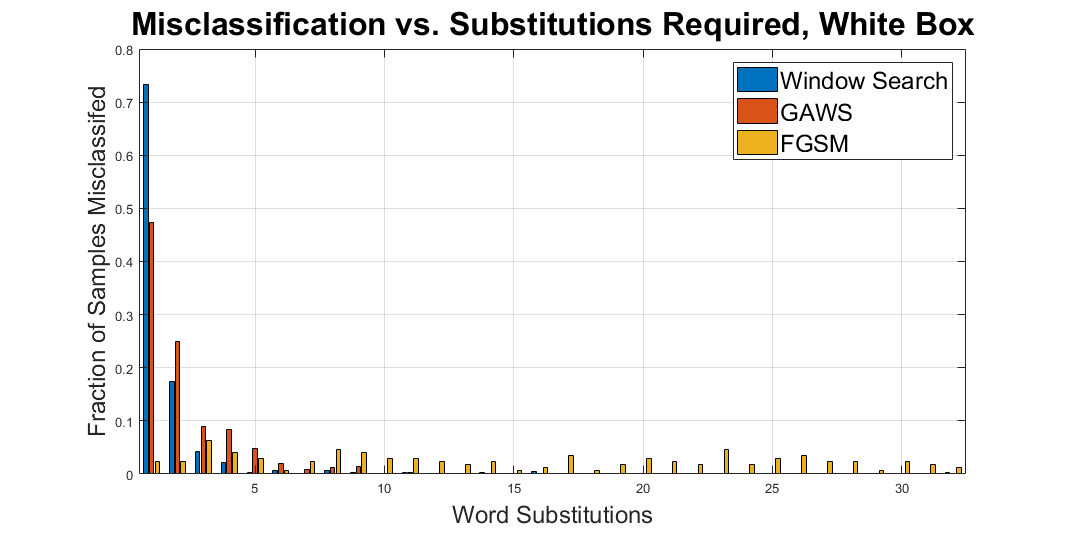
\includegraphics[width=\textwidth]{pmf_white.png}
    \caption{The x-axis represents the number of word substitutions used to change the fraction of samples represented by the y-axis.}
    \label{fig:whitepmf}
\end{figure}

\begin{figure}
    \centering
    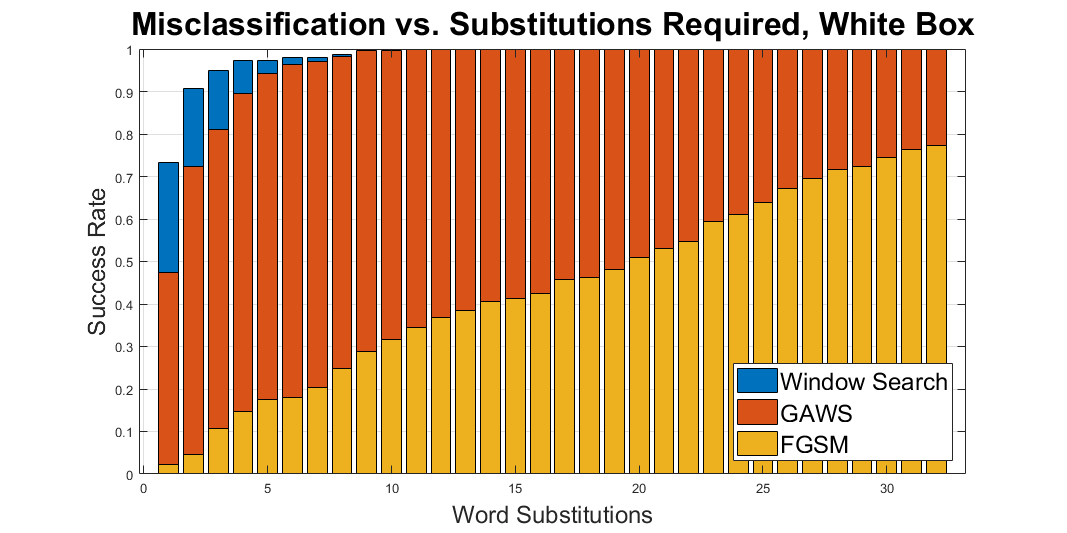
\includegraphics[width=\textwidth]{cdf_white.png}
    \caption{The y-axis represents the total fraction of samples can be successfully misclassified given the number of substitutions on the x-axis.  This is the accumulation of the graph in figure \ref{fig:whitepmf}}
    \label{fig:whitecdf}
\end{figure}

\begin{figure}
    \centering
    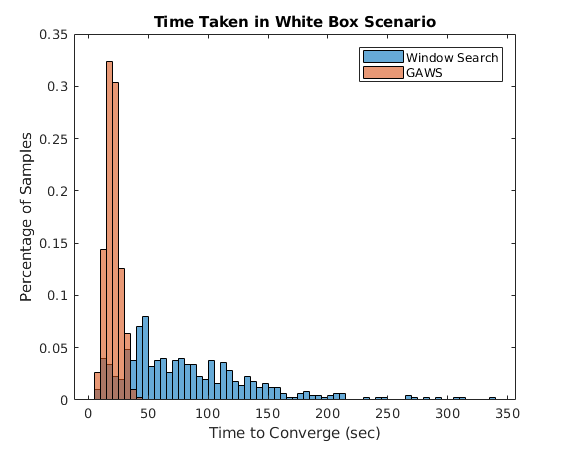
\includegraphics[width=\textwidth]{timewhite.png}
    \caption{Time taken per sample for WS and GAWS algorithms.}
    \label{fig:whitetime}
\end{figure}

\section{Gray Box}
This experiment assumes that all hyperparameters of the model being attacked are known.  In order to attack the model, we trained a second neural network with identical hyperparameters.  Because stochastic gradient descent has random components, the models will likely have very different weights by the end of training.  We infer and search on our stand-in model and then infer on the model under attack to check if it was successfully caused to misclassify the sample.  If the model under attack misclassifies the text sample to begin with, it is not considered.

\begin{table}
\centering
\begin{tabular}{ |c|c|c|c|c| } \hline
& Mean & Median & Mode & Failures\\ \hline
FGSM & 43.42 & 32 & 6 & 1\\ \hline
GAWS & 10.06 & 3 & 1 & 1\\ \hline
WS & 5.86 & 2 & 1 & 0\\ \hline
\end{tabular}
\caption{Summary statistics for the gray box experiment.  These numbers correspond to the full distributions visualized in figure \ref{fig:graypmf}.  Failures are not counted toward mean, median, nor mode.}
\label{tab:graysum}
\end{table}
\begin{figure}
    \centering
    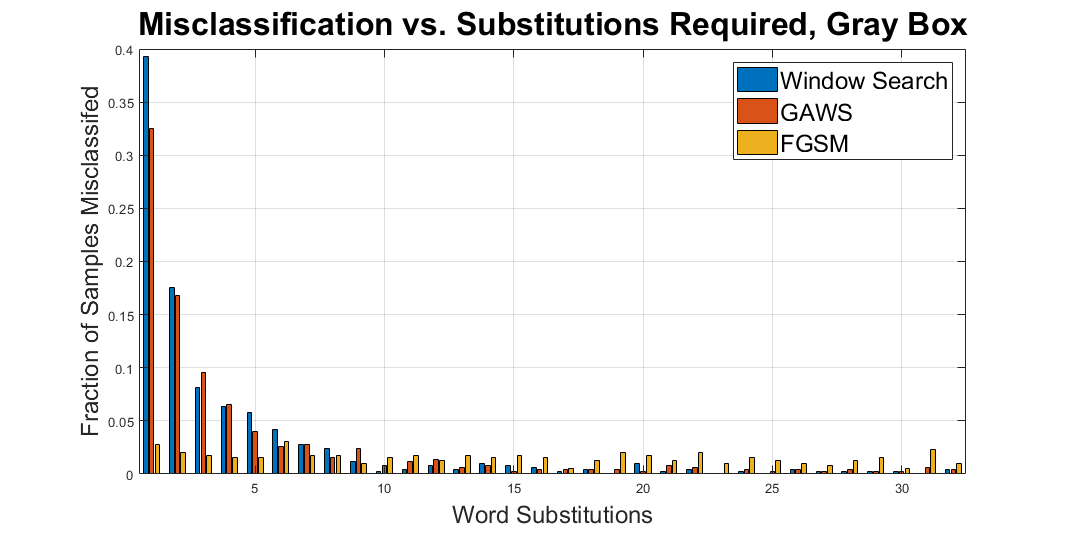
\includegraphics[width=\textwidth]{pmf_gray.png}
    \caption{The x-axis represents the number of word substitutions used to change the fraction of samples represented by the y-axis.}
    \label{fig:graypmf}
\end{figure}

\begin{figure}
    \centering
    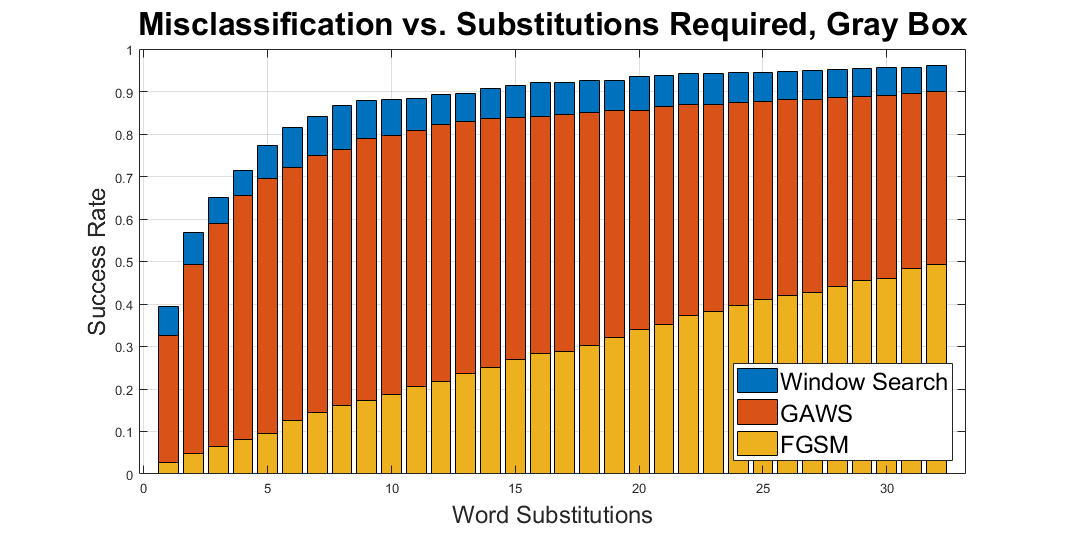
\includegraphics[width=\textwidth]{cdf_gray.png}
    \caption{The y-axis represents the total fraction of samples can be successfully misclassified given the number of substitutions on the x-axis.  This is the accumulation of the graph in figure \ref{fig:graypmf}}
    \label{fig:graycdf}
\end{figure}

Table \ref{tab:graysum} shows that performance of the algorithms is significantly degraded if the exact weights are unknown.  The average number of word replacements required to change classification increased by a factor of roughly 4.5 and 3.25 for GAWS and WS respectively.  FGSM, on the other hand worsened by a factor less than 2.  Even though GAWS and WS decreased in performance more than FGSM, they still far outperformed it, even if it is given the benefit of a white box attack.

Both Table \ref{tab:graysum} and figure \ref{fig:graypmf} show, however, that most of the samples can be successfully attacked by changing just two or three words.  These results indicate that the described algorithms do not exactly attack just one model with one set of weights, but exhibit some amount of transferability.  Figure \ref{fig:graycdf} shows that window search consistently outperforms GAWS in terms of the number of replacements required.  The shape of the WS and GAWS sequences in \ref{fig:graypmf} appear to be roughly exponential toward the start and flatten out further away.  As in the white box scenario, FGSM seems to have a fairly constant distribution and therefore linear cumulative distribution.

\section{Black Box}
This experiment assumes that no details of the model are known, in particular the hyperparameters are unknown.  In order to evaluate performance under this condition, we determine word substitutions using an RNN with a hidden layer of size 16 and attack an RNN with a hidden layer size of 8.
\begin{table}
\centering
\begin{tabular}{ |c|c|c|c|c| } \hline
& Mean & Median & Mode & Failures\\ \hline
FGSM & 43.42 & 32 & 6 & 0\\ \hline
GAWS & 10.16 & 2 & 1 & 5\\ \hline
WS & 7.16 & 2 & 1 & 0\\ \hline
\end{tabular}
\caption{Summary statistics for the black box experiment.  These numbers correspond to the full distributions visualized in figure \ref{fig:blackpmf}.  Failures are not counted toward mean, median, nor mode.}
\label{tab:blacksum}
\end{table}
\begin{figure}
    \centering
    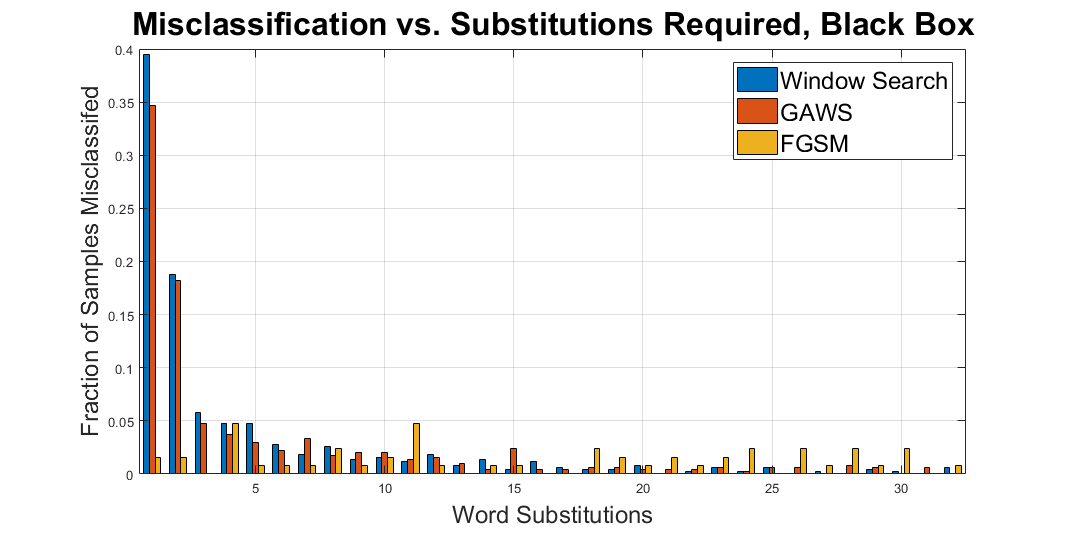
\includegraphics[width=\textwidth]{pmf_black.png}
    \caption{The y-axis represents the fraction of samples which were misclassified given the number of substitutions on the x-axis.}
    \label{fig:blackpmf}
\end{figure}

\begin{figure}
    \centering
    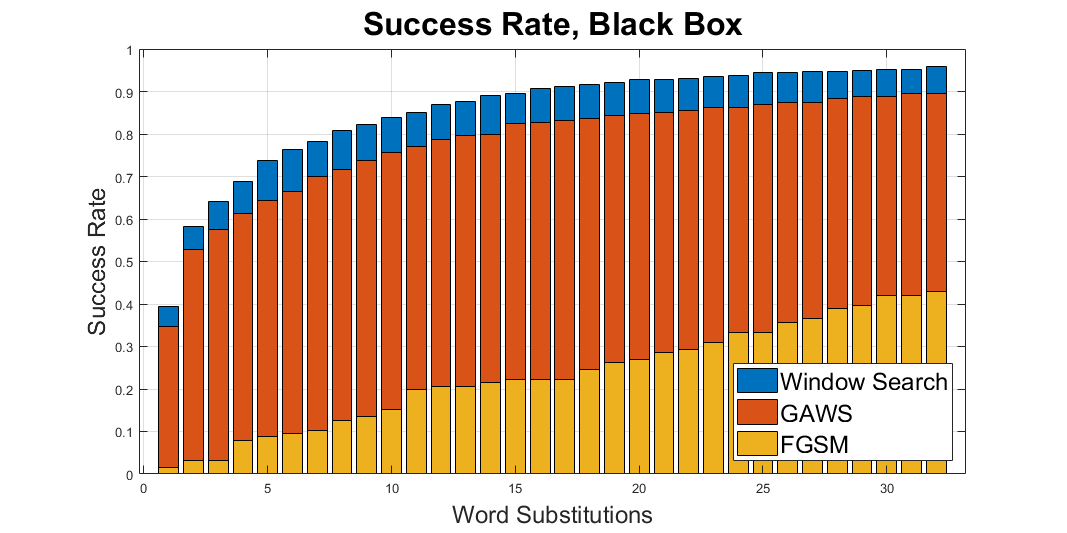
\includegraphics[width=\textwidth]{cdf_black.png}
    \caption{The y-axis represents the total fraction of samples can be successfully misclassified given the number of substitutions on the x-axis.  This is the accumulation of the graph in figure \ref{fig:blackpmf}}
    \label{fig:blackcdf}
\end{figure}

Table \ref{tab:blacksum} shows that there are significantly more failures for the GAWS algorithm, and slightly worse performance for window search algorithm.  Otherwise the statistics and figures were mostly unaffected.  None the less, this shows that our methods are viable even in black box scenarios, with window search achieving better performance than FGSM, even if it is afforded white box performance.

Note that while the cumulative distribution in figure \ref{fig:blackcdf} looks identical to the one in figure \ref{fig:graycdf}, it is only a representation of the first 32 values.  In fact, large values far in the tail of the distribution contribute a significant amount to the sample mean.  Because the sample size is a relatively small value of $500$, it is not clear whether this is significant or just statistical noise.
